\section{Big Data Analysis}

Big data analytics is where advanced analytic techniques operate on big data sets. Hence, big data
analytics is really about two things — \textit{big data} and \textit{analytics}.



\subsection{Big Data}

As the name suggests, big data is a large amount of data. There are other important attributes of big data. These are:  data variety and data velocity.

Thus we can define big data using 3 V's: \textit{volume}, \textit{variety}, and \textit{velocity} as showin in figure \ref*{bigData}.

\begin{figure}[h]
    \centering
    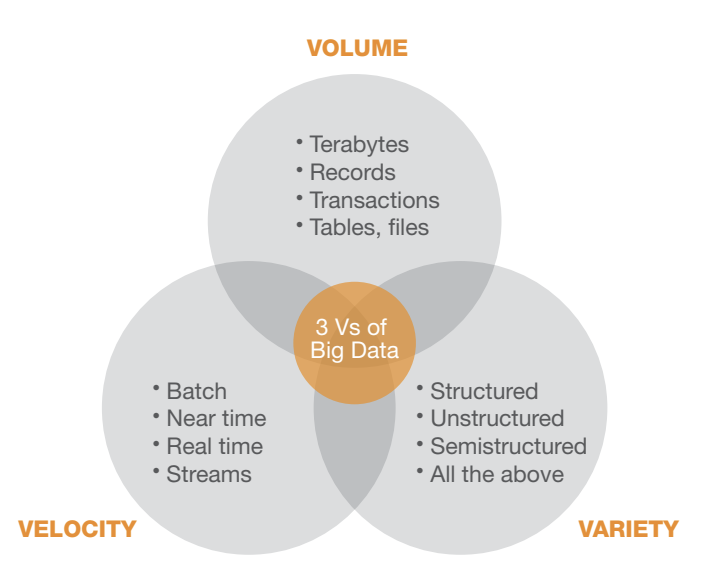
\includegraphics[width=0.5\textwidth]{images/big_data.png}
    \caption{Big Data: 3 V's \autocite{3vbigdata}}
    \label{bigData}
\end{figure}

Beyond these three V's, Big Data is also about how complicated the computing
problem is. Given the number of variables and number of data points for analysing the maritime shipping data. It is a very complicated problem.
Thus, in addition to the three V's identified by IBM, it would also be necessary to take complexity into account as shown in figure \ref*{bigDataComplex} \autocite{pence2014big}.

\begin{figure}[h]
    \centering
    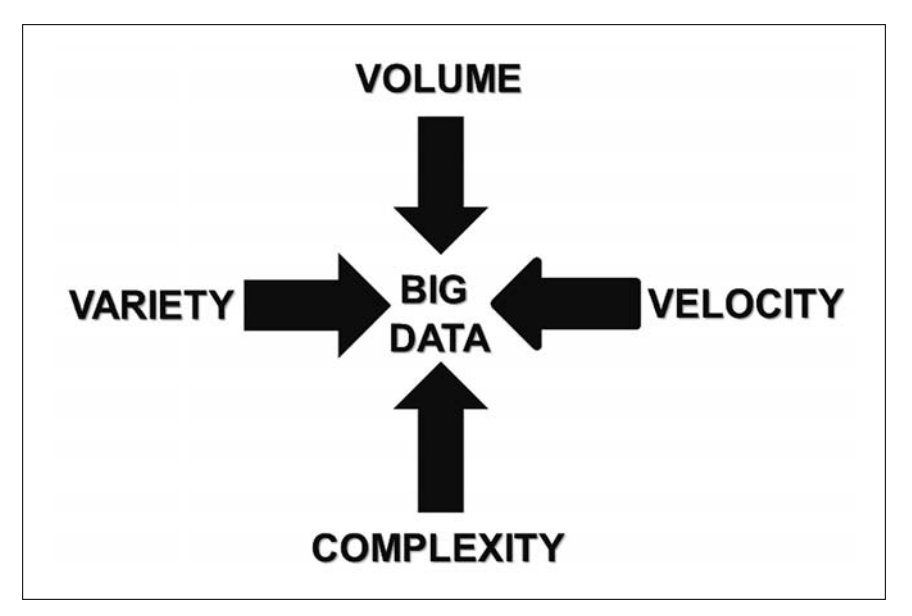
\includegraphics[width=0.5\textwidth]{images/big_data_complex.png}
    \caption{Big Data: Beyong 3 V's - volume, velocity,
        variety, and complexity}
    \label{bigDataComplex}
\end{figure}


\subsection{What is Big Data Analytics?}

Big data analytics is the process of examining large and varied data sets to uncover hidden patterns, unknown correlations, market trends, customer preferences and other useful information that can help organizations make more-informed business decisions.

Thus, Data analytics revolves around deriving valuable knowledge and meaningful insights from extensive sets of data.
This process involves crafting hypotheses, often rooted in gathered experiences and uncovering correlations between variables, sometimes even through serendipitous discoveries.
Data analytics can be classified into four distinct types \autocite{rajaraman2016big}:

\subsubsection{1. Descriptive Analytics}

Descriptive analytics focuses on explaining past events and presenting them in a comprehensible manner.
The collected data is structured into visual aids like bar charts, graphs, pie charts, maps, and scatter diagrams, facilitating easy interpretation that offers insights into the data's implications.
This mode of data representation is often termed a dashboard, reminiscent of a car's dashboard that provides details such as speed, engine status, fuel levels, and distance traveled.
A classic instance of descriptive analytics involves displaying population census data, which categorizes a nation's population by gender, age brackets, education, income, population density, and similar criteria \autocite{rajaraman2016big}.

\subsubsection{2. Predictive Analytics}

Predictive analytics extends beyond existing data to forecast forthcoming events.
It anticipates what is likely to occur in the immediate future.
Techniques like time series analysis utilizing statistical methods, neural networks, and machine learning algorithms are employed for this extrapolation.
A significant application of predictive analytics is seen in marketing, where it understands customer preferences and needs.
For instance, when purchasing shoes online, an advertisement for socks may appear.
Another prevalent application is in orchestrating election campaigns.
This involves gathering diverse data, such as the demographics of voters in different areas and their perceived needs like infrastructure and local concerns \autocite{rajaraman2016big}.

\subsubsection{3. Prescriptive Analytics}

This process detects opportunities for enhancing existing solutions by analyzing collected data.
Essentially, it guides us on the actions to undertake in order to accomplish a particular objective.
An illustrative instance is observed in the aviation industry where airlines determine seat pricing through analysis of historical travel patterns, popular travel origins and destinations, significant events, holidays, and more.
This approach is employed to optimize profit generation \autocite{rajaraman2016big}.

\subsubsection{4. Exploratory or Discovery Analytics}

This process uncovers unforeseen connections among variables within extensive datasets.
The collection and analysis of data from diverse sources opens up new avenues for gaining insights and making serendipitous discoveries.
One of its major applications involves the identification of patterns in customers' behavior by companies through sources like feedback, tweets, blogs, Facebook data, emails, and sales trends.
By deciphering customer behavior, companies can potentially predict actions like renewing a magazine subscription, switching mobile phone service providers, or canceling a hotel reservation. Armed with this information, companies can devise appealing offers aimed at altering the anticipated course of action by the customer \autocite{rajaraman2016big}.